\chapter{Weryfikacja i walidacja}
\label{ch:06}
Weryfikacja pracy kompilatora pod kątem poprawności generowanego kody wynikowego wymagała podzielenia procesu testowania na kilka etapów zależnych od implementowanej części kompilatora. W ich skład wchodzą:
\begin{itemize}
\item kontrola poprawności pracy analizy leksykalnej i syntaktycznej,
\item kontrola poprawności generowanego drzewa syntaktycznego,
\item weryfikacja pracy analizatora semantycznego,
\item weryfikacja poprawności generowanego kodu pośredniego,
\item weryfikacja poprawności generowanego kodu wynikowego dla docelowej platformy.
\end{itemize}
Ponadto kod wynikowy był testowany na płytce rozwojowej Arduino Pro Mini wyposażonej w mikrokontroler ATmega328P.

\section{Kontrola analizatora leksykalnego i syntaktycznego}
Wykorzystanie języka Java do budowy kompilatora pozwoliło na łatwe kontrolowanie poprawności implementacji poprzez uprzednie zdefiniowanie interfejsów i klas. W efekcie, przy użyciu błędnych klas w definicjach leksykalnych lub syntaktycznych, kompilator języka Java zgłaszał stosowne błędy o niezgodności typów. Podejście to było pomocne szczególnie w trakcie implementacji gramatyki języka, ze względu na wymóg stosowania ściśle wybranych klas w konstruktorach elementów drzewa syntaktycznego.

Narzędzia JFlex i GNU Bison udostępniają dodatkowe techniki pomagające w rozwiązywaniu problemów. JFlex implementuje system kontroli poprawności składni zgłaszający odpowiednie wyjątki w przypadku błędów w definicji. Ponadto dzięki trybowi pracy niezależnej (ang. \english{standalone}), możliwe było zweryfikowanie poprawności generowanych tokenów poprzez podanie ich na wejściu programu.
GNU Bison prócz mechanizmowi zgłaszania wyjątków w trakcie budowania kompilatora, pozwala także na wygenerowanie reprezentacji reguł języka w formie tekstowej. Dzięki temu możliwa była identyfikacja konflików w implementowanej gramatyce i ich naprawa. Reprezentacja tekstowa była przydatna w szczególności podczas naprawy błędów związanych ze złym priorytetem operacji arytmetycznych.
\ksremark{W Bisonie da się sprawdzić, czy są konflikty w gramatyce. Sprawdził Pan to?} \textit{Tak}

\section{Poprawność drzewa syntaktycznego}
W celu sprawdzenia poprawności generowanego drzewa syntaktycznego przez analizator syntaktyczny wykorzystano wbudowany w środowisko programistyczne VSCodium debuger. Ze względu na obiektowe podejście do problemu budowy drzewa syntaktycznego, narzędzie to pozwoliło na łatwe przeglądanie aktualnie wygenerowanej struktury drzewa w formie listy. Proces kontroli drzewa syntaktycznego przedstawia rysunek \ref{fig:vscodium-debug-ast}. Proces ten wymagał napisania odpowiednich scenariuszy testowych i krokowe przejście narzędziem debugującym przez program kompilatora. W trakcie procesu weryfikowano zgodność struktur drzewa wraz ze stanami zmiennych wiążących między sobą elementy drzewa i poprawność zgłaszanych wyjątków w przypadku napotkania stanów niedozwolonych.

\begin{figure}
\centering
	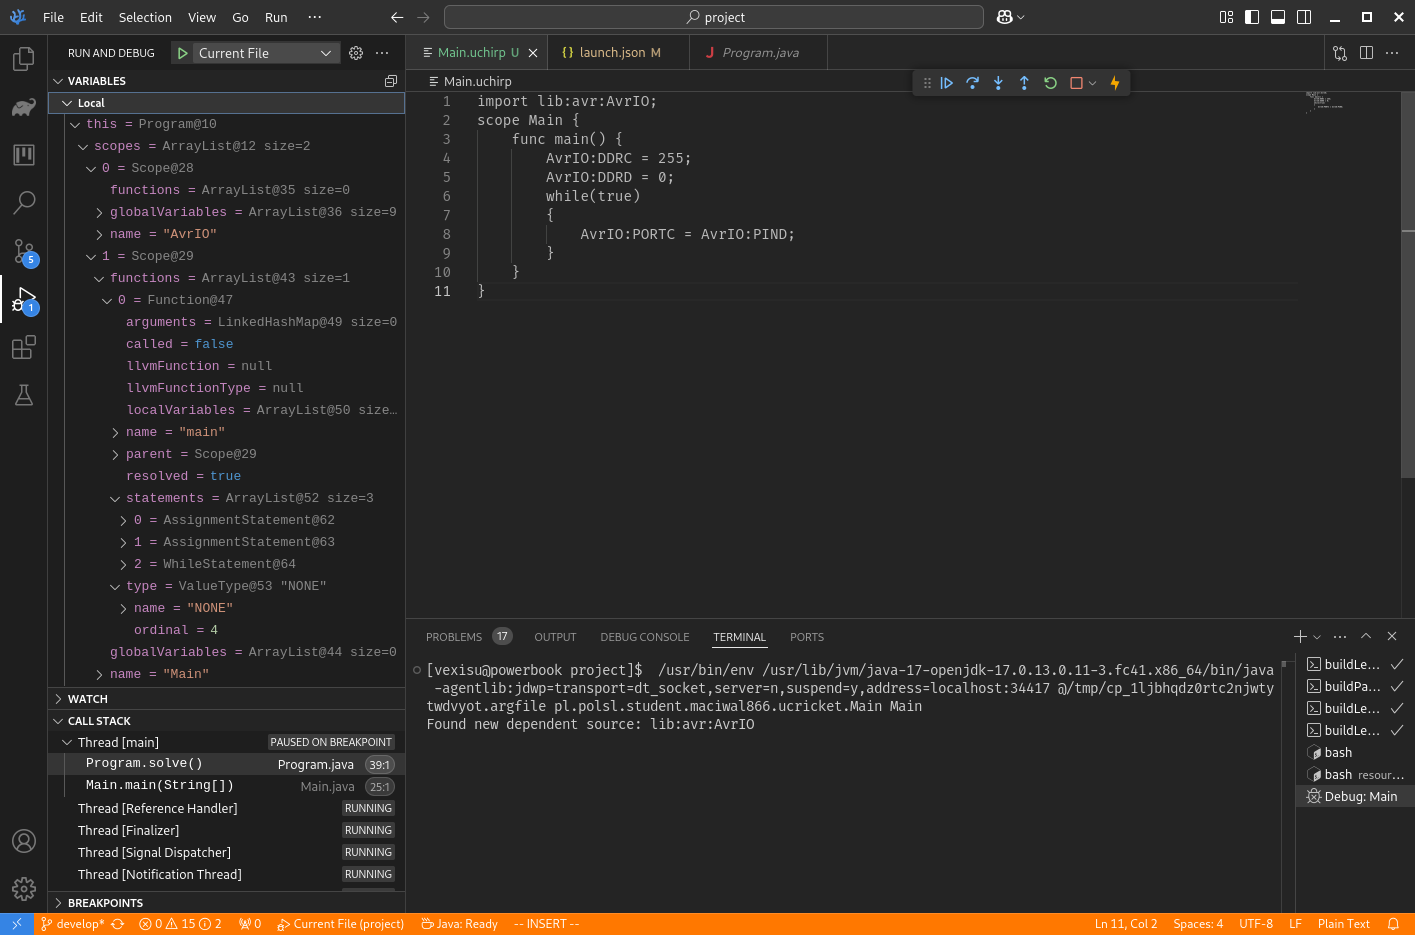
\includegraphics[width=1\textwidth]{graf/vscodium-debug-ast.png}
	\caption{Proces kontroli drzewa syntaktycznego za pomocą debugera wbudowanego w środowisko VSCodium.}
\label{fig:vscodium-debug-ast}
\end{figure}

\section{Poprawność generowanego kodu pośredniego}
Narzędzie LLVM posiada wbudowany system kontroli poprawności budowanej reprezentacji pośredniej. Odpowiada za to odpowiednia funkcja \lstinline|LLVMVerifyModule()| dostarczana przez API (ang. \english{application programming interface}), przedstawiona w kodzie źródłowym \ref{lst:ir-verify}. Wykorzystanie jej w połączeniu z funkcją \lstinline|LLVMDisposeMessage()| pozwala na weryfikację błędów w budowanej reprezentacji pośredniej. W szczególnych przypadkach, wymagane było krokowe przejście przez program narzędziem do debugowania, np. podczas przekazania nieodpowiedniej referencji typu zawartej w klasie \lstinline|LLVMTypeRef|, powodując tym samym błąd naruszenia ochrony pamięci.

\begin{lstlisting}[caption={Kod wywołujący kontrolę generowanej reprezentacji pośredniej.}, label={lst:ir-verify}]
var moduleMessage = new PointerPointer<BytePointer>(1);
LLVMVerifyModule(module, 0, moduleMessage);
LLVMDisposeMessage(moduleMessage.get(BytePointer.class)); 
\end{lstlisting}

Kolejnym mechanizmem pozwalającym na sprawdzenie poprawności kodu pośredniego było wygenerowanie jego reprezentacji w formie tekstowej przy użyciu funkcji \mbox{\lstinline|LLVMDumpModule()|.} Przekazuje ona na wyjście programu kompilatora odpowiednio sformatowaną reprezentację kodu pośredniego, którą można porównać z przygotowanym kodem testowym. Rysunek \ref{fig:ir-module-dump} przedstawia wygenerowaną reprezentację pośrednią wraz z testowanym kodem.

\begin{figure}
\centering
	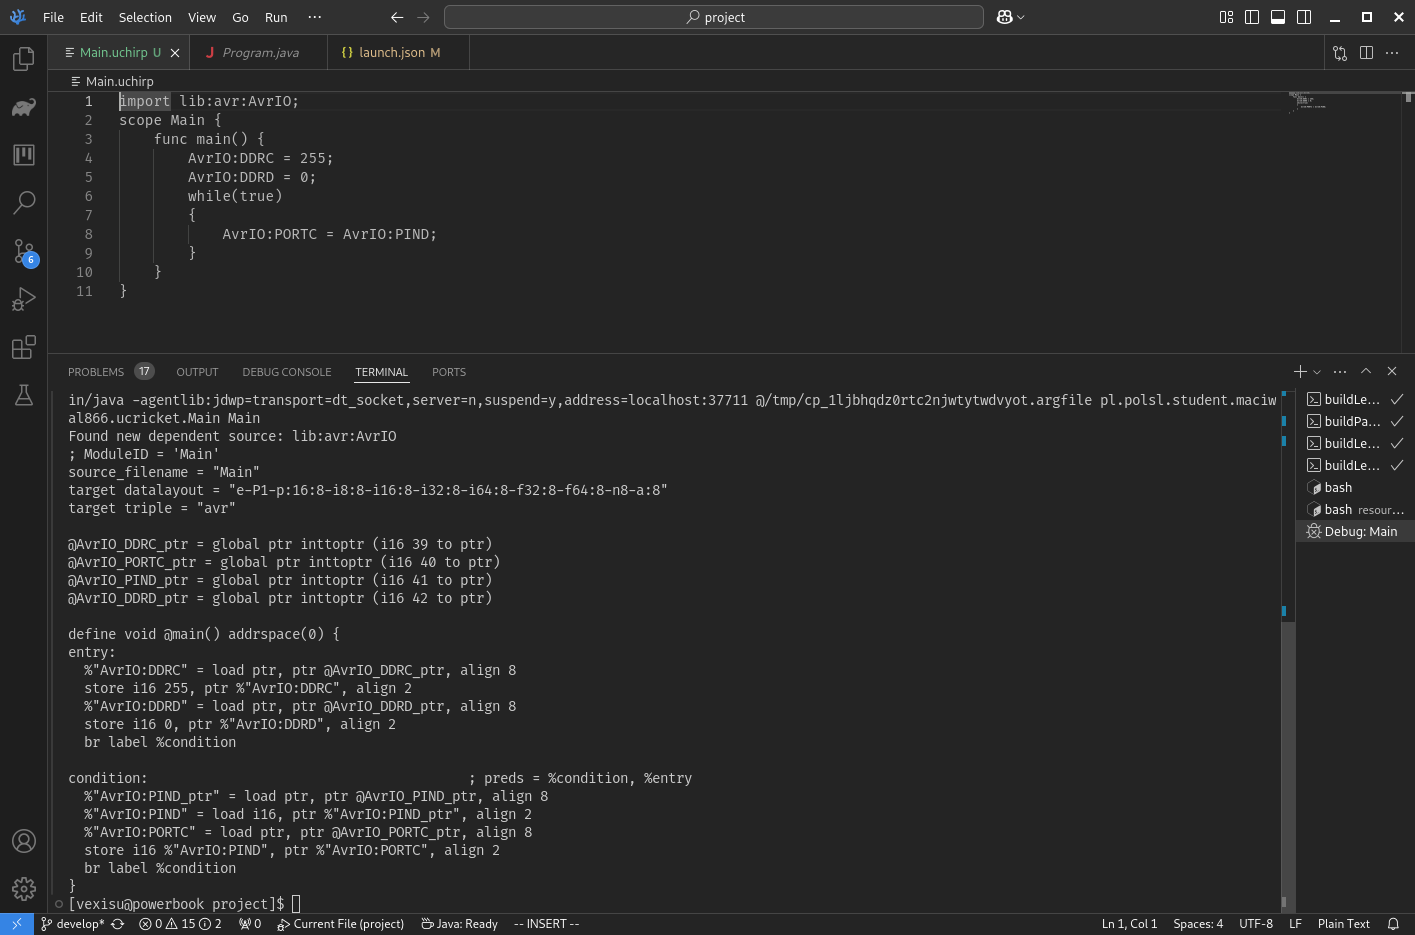
\includegraphics[width=1\textwidth]{graf/ir-module-dump.png}
	\caption{Testowy kod źródłowy wraz z jego reprezentacją pośrednią wygenerowaną przez LLVM.}
	\label{fig:ir-module-dump}
\end{figure}

\section{Poprawność kodu dla platformy wynikowej}
W trakcie generowania kodu wynikowego z poziomu narzędzia LLVM otrzymywany jest kod w języku Assembly. Jest to ostateczna czytelna forma programu dostępna dla użytkownika kompilatora. Na tym etapie kompilacji możliwe było sprawdzenie poprawności pogramu pod względem zarządzania pamięcią i wykonywanych instrukcji na procesorze mikrokontrolera. Kod języka Assembly jest dużo bardziej szczegółowy niż reprezentacja pośrednia dostarczana z narzędzia LLVM. Rysunek \ref{fig:compiled-asm-vs-ir} przedstawia finalny kod wygenerwoany przez LLVM wraz z jego reprezentacją pośrednią. 

\begin{figure}
	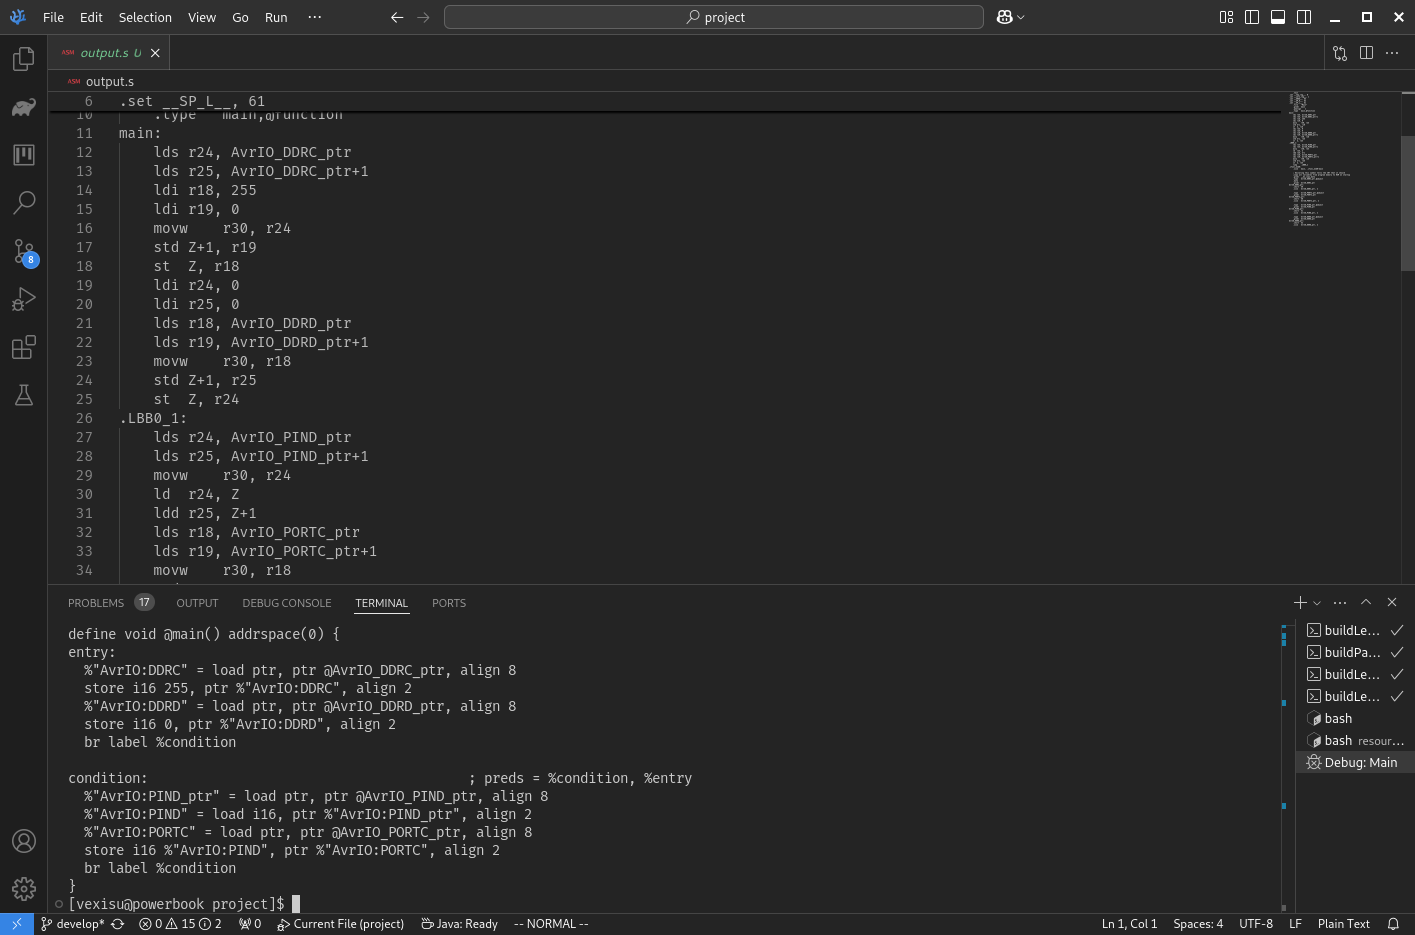
\includegraphics[width=1\textwidth]{graf/compiled-asm-vs-ir.png}
	\caption{Kod wynikowy w języku Assembly wraz z jego reprezentacją pośrednią.}
	\label{fig:compiled-asm-vs-ir}
\end{figure}

Kod binarny dla platformy docelowej uzyskany zostaje poprzez kompilację przy użyciu narzędzia avr-gcc. Testowanie pliku binarnego wymaga użycia odpowiedniego narzędzia pozwalającego na odczytanie instrukcji zakodowanych w formacie zrozumiałym dla mikrokontrolera. Do tego zadania użyto narzędzie Cutter. Jego głównym zastosowaniem jest inżyniera wsteczna kodu binarnego. Oferuje ono także debugowanie skompilowanych programów poprzez wbudowany symulator. Instrukcje programu prezentowane są wraz z odpowiednimi komentarzami akcji. Możliwe jest też przedstawienie kodu jako graf przepływu (rysunek \ref{fig:cutter-graph}). Dzięki niemu możliwa była krokowa analiza zachowania programu wraz z podglądem pamięci i rejestrów symulowanego mikrokontrolera. Rysunek \ref{fig:cutter-debug} prezentuje proces debugowania kodu wynikowego w programie Cutter. 

\begin{figure}
	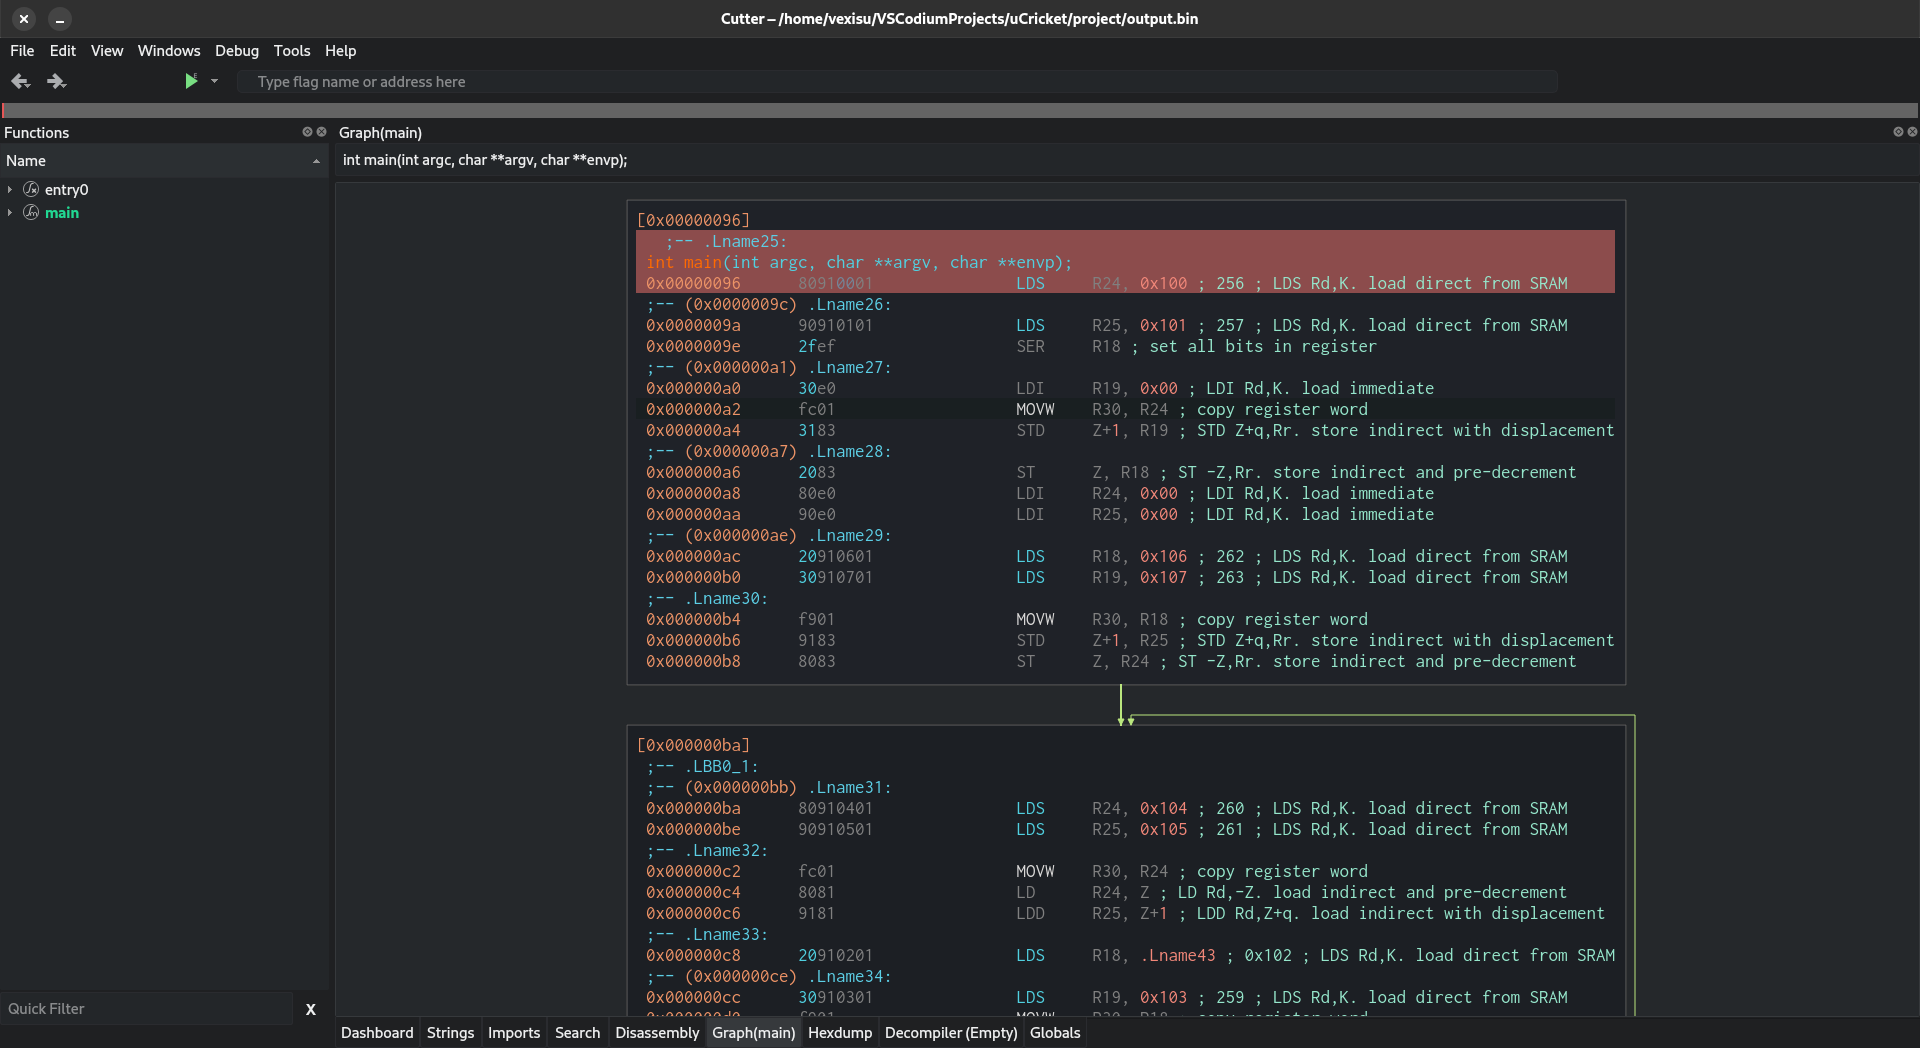
\includegraphics[width=1\textwidth]{graf/cutter-graph.png}
	\caption{Kod wynikowy w formie grafu prepływu prezentowanego w programie Cutter.}
	\label{fig:cutter-graph}
\end{figure}

\begin{figure}
	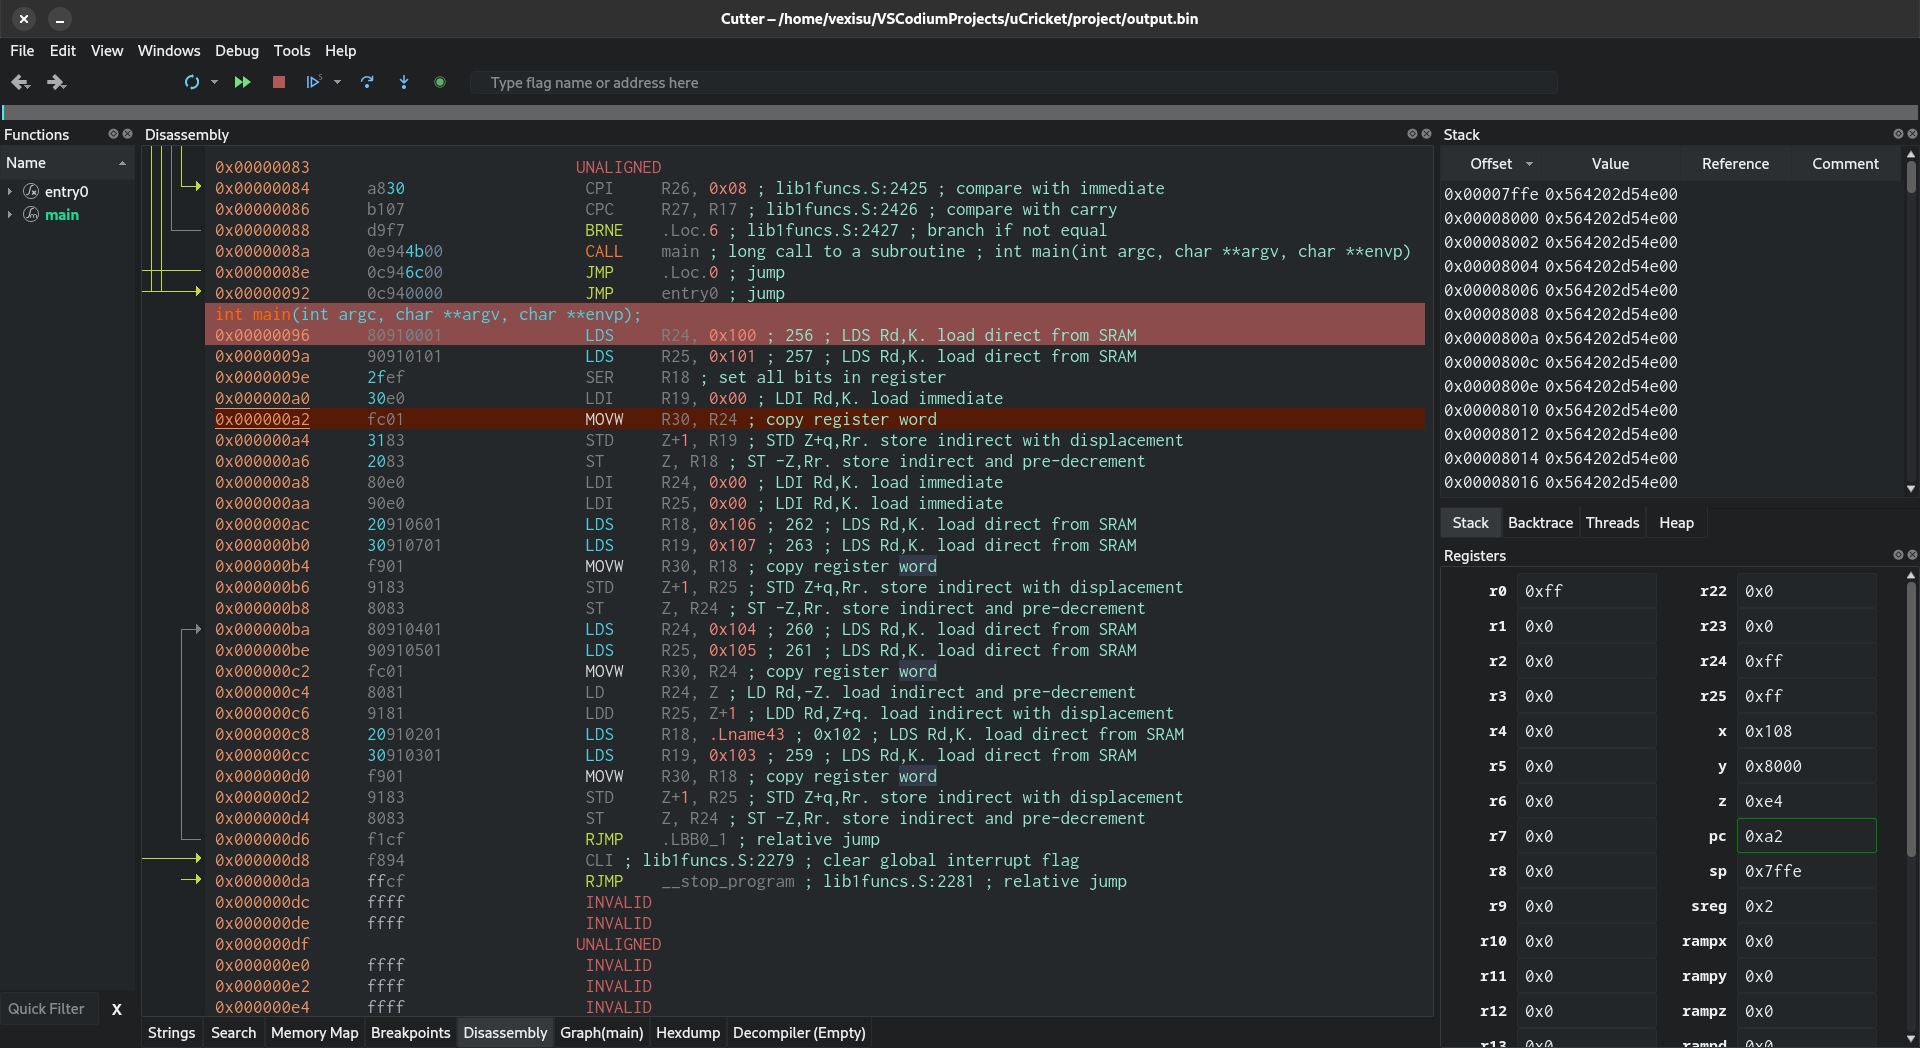
\includegraphics[width=1\textwidth]{graf/cutter-debug.png}
	\caption{Proces debugowania kodu wynikowego w programie Cutter.}
	\label{fig:cutter-debug}
\end{figure}

Program wynikowy został także przetestowany na platformie docelowej skłającej się z płytki rozwojowej Arduino Mini Pro posiadającej mikrokontroler ATmega328P. Prezentowany program wymagał także skonstruowanie układu z diod, przełączników i odpowiednich komponentów pasywnych. Rysunki \ref{fig:schematic} i \ref{fig:electronics} prezentują schemat i układ na którym testowano program. Programowanie mikrokontrolera odbyło się przy użyciu programatora USBasp.

\begin{figure}
	\textit{Tutaj zostanie dodany schemat}
	\caption{Schemat układu wykorzystanego do przetestowania programu.}
	\label{fig:schematic}
\end{figure}

\begin{figure}
	\textit{Tutaj zostanie dodane zdjęcie układu}
	\caption{Układ przeznaczony do testowania programu.}
	\label{fig:electronics}
\end{figure}

%\begin{itemize}
%\item sposób testowania w ramach pracy (np. odniesienie do modelu V)
%\item organizacja eksperymentów
%\item przypadki testowe zakres testowania (pełny/niepełny)
%\item wykryte i usunięte błędy
%\item opcjonalnie wyniki badań eksperymentalnych
%\end{itemize}

%\begin{table}
%\centering
%\caption{Nagłówek tabeli jest nad tabelą.}
%\label{id:tab:wyniki}
%\begin{tabular}{rrrrrrrr}
%\toprule
%	         &                                     \multicolumn{7}{c}{metoda}                                      \\
%	         \cmidrule{2-8}
%	         &         &         &        \multicolumn{3}{c}{alg. 3}        & \multicolumn{2}{c}{alg. 4, $\gamma = 2$} \\
%	         \cmidrule(r){4-6}\cmidrule(r){7-8}
%	$\zeta$ &     alg. 1 &   alg. 2 & $\alpha= 1.5$ & $\alpha= 2$ & $\alpha= 3$ &   $\beta = 0.1$  &   $\beta = -0.1$ \\
%\midrule
%	       0 &  8.3250 & 1.45305 &       7.5791 &    14.8517 &    20.0028 & 1.16396 &                       1.1365 \\
%	       5 &  0.6111 & 2.27126 &       6.9952 &    13.8560 &    18.6064 & 1.18659 &                       1.1630 \\
%	      10 & 11.6126 & 2.69218 &       6.2520 &    12.5202 &    16.8278 & 1.23180 &                       1.2045 \\
%	      15 &  0.5665 & 2.95046 &       5.7753 &    11.4588 &    15.4837 & 1.25131 &                       1.2614 \\
%	      20 & 15.8728 & 3.07225 &       5.3071 &    10.3935 &    13.8738 & 1.25307 &                       1.2217 \\
%	      25 &  0.9791 & 3.19034 &       5.4575 &     9.9533 &    13.0721 & 1.27104 &                       1.2640 \\
%	      30 &  2.0228 & 3.27474 &       5.7461 &     9.7164 &    12.2637 & 1.33404 &                       1.3209 \\
%	      35 & 13.4210 & 3.36086 &       6.6735 &    10.0442 &    12.0270 & 1.35385 &                       1.3059 \\
%	      40 & 13.2226 & 3.36420 &       7.7248 &    10.4495 &    12.0379 & 1.34919 &                       1.2768 \\
%	      45 & 12.8445 & 3.47436 &       8.5539 &    10.8552 &    12.2773 & 1.42303 &                       1.4362 \\
%	      50 & 12.9245 & 3.58228 &       9.2702 &    11.2183 &    12.3990 & 1.40922 &                       1.3724 \\
%\bottomrule
%\end{tabular}
%\end{table}  
%
